\documentclass{beamer}
\usetheme{metropolis}
%\usecolortheme[named=Blue]{structure}
%\useoutertheme{infolines}
\usepackage{amsmath,amssymb,amsfonts,amsthm}
\usepackage{movie15}
\usepackage{multirow}
\usepackage{hhline}
\usepackage{multicol}
\usepackage[font=scriptsize]{subcaption}
\usepackage[font=scriptsize]{caption}


%\usetheme{}
%\usetheme{Boadilla}
%\usetheme{Madrid}
%\usetheme{Pittsburgh}
%\usetheme[height=7mm]{Rochester}
%\usetheme{Copenhagen}
%\usetheme{Warsaw}
%\usetheme{Singapore}
%\usetheme{Malmoe}

\setbeamertemplate{items}[rectangle]
\setbeamertemplate{blocks}[rounded][shadow=false]
\setbeamertemplate{navigation symbols}{}

\usepackage{bbding}

%\graphicspath{{Figs/}}


%------------------------------------------------------------------------------

\def\div{\nabla\cdot}
%\def\Div{\text{{\rm div}}}
\def\curl{\nabla\times}
\def\Curl{\text{{\rm curl}}}
\def\<{\langle}
\def\>{\rangle}


\def\E{{\cal E}}
\def\SS{{\cal S}}

\def\hE{\hat E}
\def\tE{\tilde E}
\def\hX{\hat\X}
\def\tX{\tilde\X}
\def\hx{\hat x}
\def\tx{\tilde x}
\def\cX{\check\X}
\def\X{{\bf x}}
\def\tu{{\bf\tilde u}}
\def\cE{\check E}
\def\D{{\bf D}}
\def\bE{{\bf E}}

\def\dt{\Delta t}
\def\ezw{\widehat{E_{w}}}
\def\ezo{\widehat{E_{o}}}
\def\de{\delta}

\def\u{{\bf u}}
\def\tu{{\bf\tilde u}}
\let\vv=\v
\def\v{{\bf v}}

\def\e{{\bf e}}
\def\u{{\mathbf u}}
\def\v{{\bf v}}
\def\x{{\bf x}}
\def\q{{\bf q}}
\def\b{{\bf b}}
\def\g{{\bf g}}
\def\z{{\bf z}}
\def\Z{{\bf Z}}
\def\t{{\bf t}}
\def\w{{\bf w}}
\def\s{{\bf s}}
\def\n{{\bf n}}
\def\f{{\bf f}}
\def\U{{\bf U}}
\def\V{{\bf V}}
\def\X{{\bf X}}
\def\M{{\bf M}}
\def\K{{\bf K}}
\def\bI{{\bf I}}
\def\r{{\bf r}}
\def\btau{\mbox{{\boldmath$\tau$}}}
\def\bxi{\mbox{{\boldmath$\xi$}}}
\def\bs{\mbox{{\boldmath$\sigma$}}}
\def\be{\mbox{{\boldmath$\epsilon$}}}
\def\bl{\mbox{{\boldmath$\lambda$}}}
\def\bmu{\mbox{{\boldmath$\mu$}}}
\def\bphi{\mbox{{\boldmath$\phi$}}}
\def\bpsi{\mbox{{\boldmath$\psi$}}}
\def\bbeta{\mbox{{\boldmath$\eta$}}}
\def\B{{\mathcal B}}
\def\d{\partial}
\def\T{{\mathcal T}}
\def\tU{{{\bf \tilde{\U}}}}
\def\tV{{{\bf \tilde{\V}}}}
\def\tv{{{\bf \tilde{\v}}}}
\def\R{{\mathbb R}}
\def\grad{\nabla}
\def\div{\grad \cdot}
\def\al{\alpha}
\def\l{\lambda}
\def\lam{\lambda}
\def\bP{\bar{P}}
\def\bS{\bar{S}}
\def\O{\Omega}
\def\G{\bf{G}}
\def\eps{\varepsilon}
\def\E{{\cal E}}
\def\Q{{\cal Q}}
\def\I{{\cal I}}
\def\<{\langle}
\def\>{\rangle}
\def\F{\mathcal F}
\def\domp{\Omega_p}

\newtheorem{proposition}{Proposition}
\newtheorem{remark}{Remark}

\newcommand {\ttt}{|\!|\!|}
\newcommand{\dd}{{\rm div}}
\newcommand{\Om}{{\Omega}}
\newcommand{\inp}[2][]{\left(#1,\, #2\right)}
\newcommand{\gnp}[2][]{\langle#1,\, #2\rangle}
\def\baru{\bar{\u}}
\def\barp{\bar{p}}

\def\width{\delta}
\def\midline{\gamma}
\def\normgama{\boldsymbol{n}}
\def\tanggama{\boldsymbol{\tau}}
\def\avgut{U_{\tau}}
\def\avgun{U_{n}}
\def\curve{\mathcal{C}}
\def\Pf{P}
\def\forcefo{\boldsymbol{f}_f}
\def\brink{\epsilon}
\def\boundo{\Gamma_1}
\def\boundt{\Gamma_2}
\def\displ{\boldsymbol{\eta}}
\def\normo{\boldsymbol{n}_1}
\def\normt{\boldsymbol{n}_2}

\def\tango{\boldsymbol{\tau}_1}
\def\tangt{\boldsymbol{\tau}_2}

\def\Red{\textcolor{Red}}
\def\Blue{\textcolor{Blue}}
\def\DarkBlue{\textcolor{DarkBlue}}
\def\Black{\textcolor{Black}}
\def\PineGreen{\textcolor{PineGreen}}
\def\OliveGreen{\textcolor{myolivegreen}}
\def\Green{\textcolor{Green}}
\def\Purple{\textcolor{Purple}}
\def\Cyan{\textcolor{Cyan}}
\definecolor{DarkBlue}{rgb}{0,0.08,0.45}
\definecolor{DarkBrown}{cmyk}{0, 0.81, 1, 0.70}

\def\Line(#1,#2)(#3,#4){\qbezier(#1,#2)(#1,#2)(#3,#4)}

\def\bK{{\bf K}}
\def\bI{{\bf I}}
\def\bT{{\bf T}}
\def\bD{{\bf D}}
\def\bA{{\bf A}}
\def\tmu{{\tilde \mu}}
\def\tlambda{{\tilde \lambda}}
\def\tr{\text{tr}}
\def\Div{\text{div}\,}

% definitions
\def\DD{\boldsymbol D}
\def\uu{\boldsymbol U}
\def\nn{\boldsymbol{n}}
\def\hnn{\hat{\boldsymbol{n}}}
\def\ttau{\boldsymbol{\tau}}
\def\httau{\hat{\boldsymbol{t}}}
\def\hGamma{\hat{\Gamma}}
\def\bilinAA{{\mathcal A}}
\def\dt{d_\tau}
\def\dtt{d_\tau}
\def\interf{\Gamma}
\def\aalpha{}

%fluid domain
\def\domf{\Omega_f}
\def\hdomf{\hat{\Omega}_f}
\def\velf{\boldsymbol{u}_f}
\def\evelf{\widehat{\boldsymbol{e}}_{v,h}}
\def\hvelf{\hat{\boldsymbol{u}_f}}
\def\bff{\boldsymbol{\varphi}_{f}}
\def\hbff{\hat{\boldsymbol{\varphi}}_{f,h}}
\def\strf{\boldsymbol{\sigma}_{f}}
\def\hstrf{\hat{\boldsymbol{\sigma}}_{f}}
\def\strfv{\boldsymbol{D}_{f}}
\def\strfp{\pf}
\def\pf{p_{f}}
\def\epf{\widehat{e}_{p,f,h}}
\def\hpf{\hat{p}_{f}}
\def\bpf{\psi_{f}}
\def\hbpf{\hat{\psi}_{f}}

% porous matrix fluid equations
\def\domp{\Omega_p}
\def\hdomp{\hat{\Omega}_p}
\def\velp{\boldsymbol{u}_p}
\def\evelp{\widehat{\boldsymbol{e}}_{q,h}}
\def\hvelp{\hat{\boldsymbol{u}_p}}
\def\bfp{{\boldsymbol{r}}}
\def\hbfp{\hat{\boldsymbol{r}}}
\def\pp{p_{p}}
\def\ppone{p_{p,1}}
\def\pptwo{p_{p,2}}
\def\epp{\widehat{e}_{p,p,h}}
\def\hpp{\hat{p}_{p}}
\def\bpp{\psi_{p}}
\def\hbpp{\hat{\psi}_{p}}
\def\velr{\boldsymbol{w}}
\def\velz{\boldsymbol{u}}
\def\hvelr{\hat{\boldsymbol{w}}}

% porous matrix solid equations
\def\strp{\boldsymbol{\sigma}_{p}}
\def\hstrp{\hat{\boldsymbol{\sigma}}_{p}}
\def\dispp{\boldsymbol{\eta}}
\def\edispp{\widehat{\boldsymbol{e}}_{\eta,h}}
\def\dotdispp{\dot{\boldsymbol{\eta}}}
\def\edotdispp{\dot{\widehat{\boldsymbol{e}}}_{\eta,h}}
\def\hdispp{\hat{\boldsymbol{\eta}}}
\def\bsp{\boldsymbol{\varphi}_{p}}
\def\dotbsp{\dot{\boldsymbol{\varphi}}_{p}}
\def\hbsp{\hat{\boldsymbol{\varphi}}_{p}}
\def\strep{\boldsymbol{\sigma}_{E}}
\def\hstrep{\hat{\boldsymbol{\sigma}}_{E}}

% fem spaces
\def\femvf{\mathbf{V}_h^f}
\def\femvp{\mathbf{V}_h^p}
\def\fempf{Q_h^f}
\def\fempp{Q_h^p}
\def\fems{\mathbf{X}_h^p}
\def\dotfems{\dot{\mathbf{X}}_h^p}
\def\hfems{\hat{\mathbf{X}}_h^p}
\def\femm{\mathbf{X}_h^m}
\def\dotfemm{\dot{\mathbf{X}}_h^m}
\def\hfemm{\hat{\mathbf{X}}_h^m}

% bilinear forms
\def\bilinasp{a_{s}}
\def\bilinbsp{b_{s}}
\def\bilinm{a_m}
\def\bilinaff{{a}_{f}}
\def\bilinbff{{b}_{f}}
\def\bilinafp{{a}_{p}}
\def\bilinbfp{{b}_{p}}
\def\bilincfp{{c}_{p}}
\def\stabffp{{s}_{f,p}}
\def\stabffv{{s}_{f,v}}
\def\stabffq{{s}_{f,q}}

% energy
\def\energyf{E_{f,h}}
\def\energys{E_{p,h}}
\def\energym{E_{m,h}}

% error
\def\errorf{\mathcal{E}_{f,h}}
\def\errors{\mathcal{E}_{p,h}}
\def\errorm{\mathcal{E}_{m,h}}

% symmetry
\def\sym{\varsigma}

% rhs
\def\fff{{\cal F}}
\def\TT{{\cal T}}


%stability analysis
\def\epsfa{\widehat{\epsilon}_f^\prime}
\def\epsfab{\widecheck{\epsilon}_f^\prime}
\def\epsfaa{\epsilon_f^{\prime\prime}}
\def\epsfaaa{\widecheck{\epsilon}_f^{\prime\prime\prime}}
\def\epsfiv{\widehat{\epsilon}_f^{\prime\prime\prime}}

\def\epspa{\epsilon_p^\prime}
\def\epspaa{\epsilon_p^{\prime\prime}}
\def\epspaaa{\epsilon_p^{\prime\prime\prime}}

% convergence analysis
\def\yy{{\boldsymbol y}_h}
\def\yysn{{\boldsymbol y}_h(t_n)}
\def\yyi{\widetilde{\boldsymbol y}}
\def\yye{\widehat{\boldsymbol y}}
\def\yyin{\widetilde{\boldsymbol y}_h^n}
\def\yyen{\widehat{\boldsymbol y}_h^n}
\def\ein{\widetilde{\boldsymbol e}_h^n}
\def\ee{\widehat{\boldsymbol E}_h}
\def\een{\widehat{\boldsymbol e}_h^n}
\def\eeN{\widehat{\boldsymbol e}_h^N}
\def\zzh{{\boldsymbol z}_h}
\def\zz{{\boldsymbol z}_h}
\def\aas{{\cal A}_h}
\def\aasi{\widetilde{\cal A}_h}
\def\aasis{\widetilde{\cal A}_h^s}
\def\aase{\widehat{\cal A}_h}
\def\rsi{\widetilde{\cal R}_h}
\def\rse{\widehat{\cal R}_h}
\def\stab{{\cal S}_h}
\def\spliterr{{\cal R}_h}

\def\maas{{\mathrm{A}}_h}
\def\maasi{\widetilde{\mathrm{A}}_h}
\def\maasis{\widetilde{\mathrm{A}}_h^s}
\def\maase{\widehat{\mathrm{A}}_h}
\def\YY{{\boldsymbol Y}}
\def\ZZ{{\boldsymbol Z}}
\def\XX{{\boldsymbol X}}
\def\FF{{\boldsymbol F}}
\def\RR{{\boldsymbol R}}

\def\sumtau{\tau \sum_{n=1}^N}

\def\gones{(s,{\textstyle\frac{-\delta(s)}{2}})}
\def\gtwos{(s,{\textstyle\frac{+\delta(s)}{2}})}


% number sets
\def\Kset{\mathbb{K}}
\def\Mset{\mathbb{M}}
\def\Nset{\mathbb{N}}
\def\Pset{\mathbb{P}}
\def\Qset{\mathbb{Q}}
\def\Rset{\mathbb{R}}
\def\Sset{\mathbb{S}}
\def\Vset{\mathbb{V}}
\def\Zset{\mathbb{Z}}

\def\Tc{\mathcal{T}}

\def\BDM{\text{BDM}}

% commands
\newcommand{\triple}[1]{|||#1|||}
\newcommand{\iii}[1]{{\left\vert\kern-0.25ex\left\vert\kern-0.25ex\left\vert #1 
		\right\vert\kern-0.25ex\right\vert\kern-0.25ex\right\vert}}

\title[The Battle of Neighborhoods]
{The Battle of Neighborhoods: \\
Exploration of Austin Food Venues}
%\institute[Pitt]{
%Department of Mathematics \\
%University of Pittsburgh \\
%}
\vskip0.3in

\date[\today]

%\include{mydefs}
\begin{document}
  \maketitle
  \begin{frame}{The city of Austin, TX}
  Demographics  of Austin:
    \begin{itemize}
    \item[\EightStarTaper] one of {\it the most rapidly growing cities} in the United States;
    \item[\EightStarTaper] steady job growth, stable housing market, desirable lifestyle and  {\it booming tech industry}.
      \end{itemize}
      \begin{figure}[ht!]
	\centering
	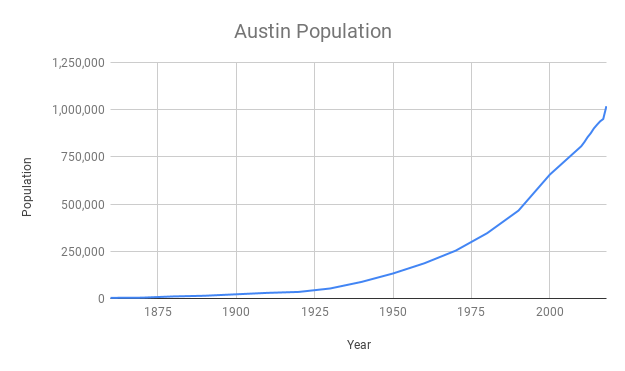
\includegraphics[width=.8\textwidth]{pics/austin_growth}
\end{figure}

  \end{frame}
 % 
    \begin{frame}{The city of Austin, TX (cont'd)}
     \begin{figure}[ht!]
	\centering
	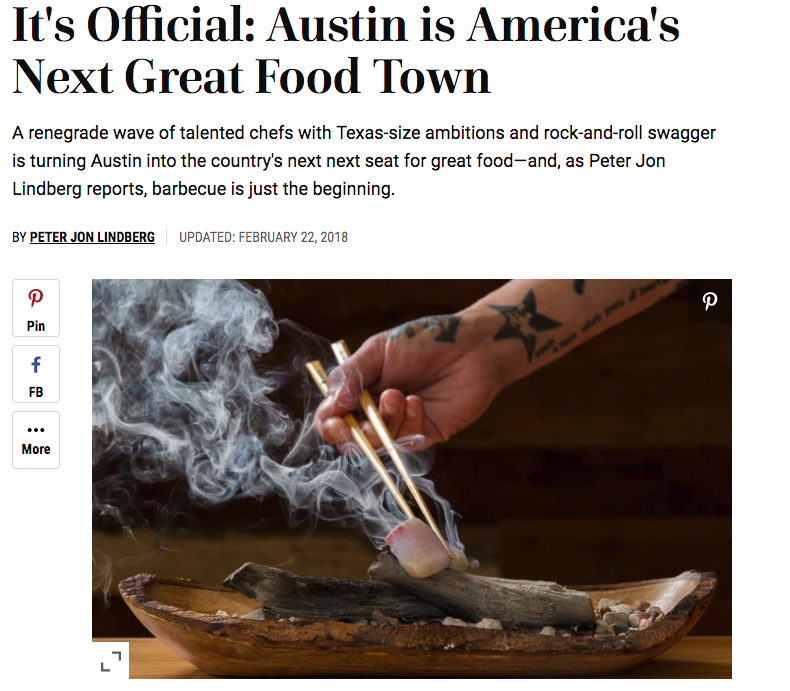
\includegraphics[width=.6 \textwidth]{pics/title}
\end{figure}
    \begin{itemize}
    \item[\EightStarTaper] synonymous with barbecue, as well as killer bars, and all manner of food trucks;
    \item[\EightStarTaper] is now becoming {\it one of the top food destination} in the US.
      \end{itemize}
  \end{frame}
  %
  \begin{frame}{Suggestion for a new business}
  \begin{center}
{\it Open a restaurant, which would feature a more
elegant selection of food and drinks, comparing to BBQ, tacos and beer, that at the same time would be
interesting and attractive for both locals and tourists.}
\end{center}
    \end{frame}
    %
     \begin{frame}{Project description}
  \begin{center}
{\bf Conduct the analysis of Austin food venues and suggest
the best unusual category for a new restaurant, together with the optimal location, based
on the additional analysis of the city's neighborhoods}, using:
\end{center}
\begin{itemize}
\item[\EightStarTaper] data, describing the current food venues available in the city;
\item[\EightStarTaper] data, summarizing the city's neighborhoods.
\end{itemize}
    \end{frame}
% 
    \begin{frame}{Neighborhoods of Austin}
 The city is split into 48 neighborhoods:   
     \begin{figure}[H]
	\centering
	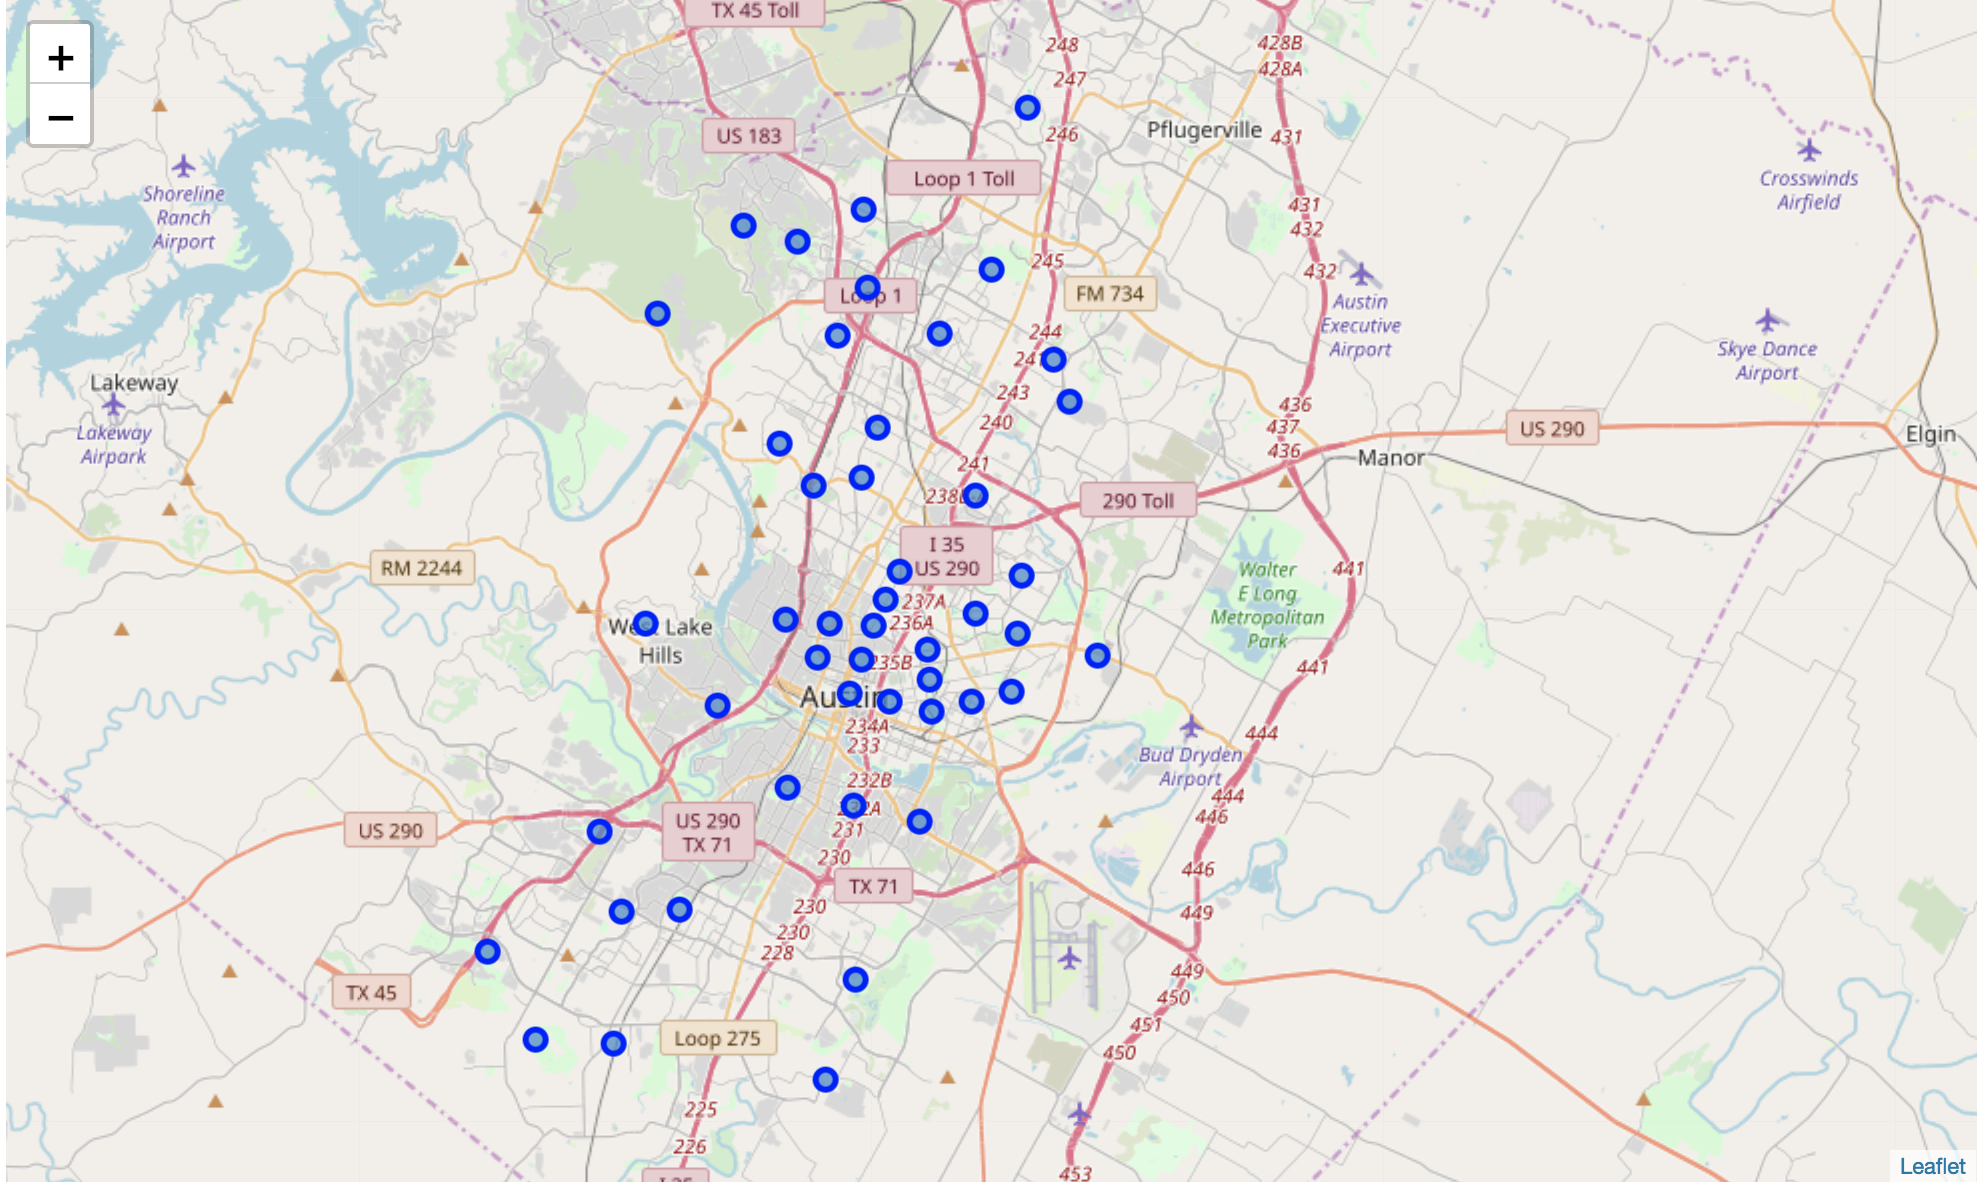
\includegraphics[width=.9\textwidth]{pics/neighborhoods}
\end{figure}
  \end{frame}
  % 
    \begin{frame}{Available food venues}
Top 20 most frequent food places in Austin:
     \begin{figure}[H]
	\centering
	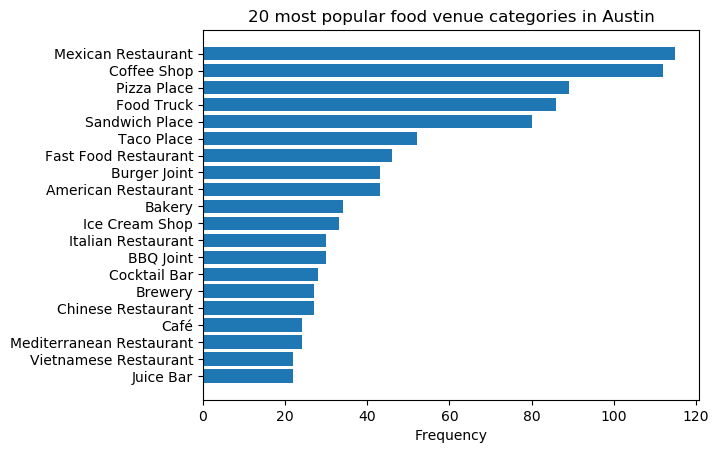
\includegraphics[width=.9\textwidth]{pics/top_20_venues}
\end{figure}
  \end{frame}
   % 
    \begin{frame}{Available food venues (cont'd)}
Bottom 20 most frequent food places in Austin:
     \begin{figure}[H]
	\centering
	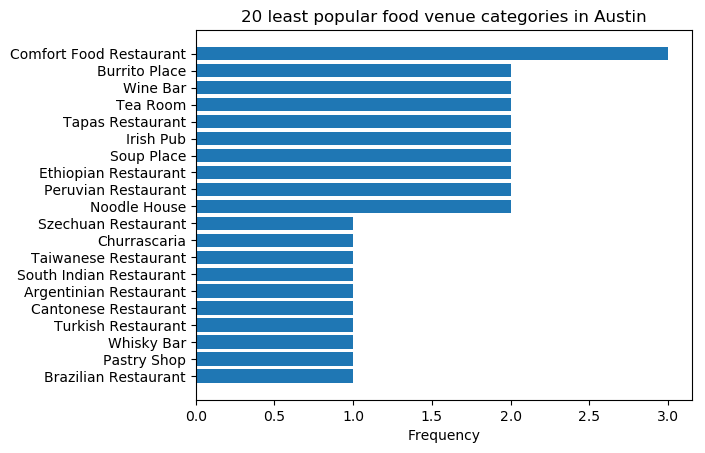
\includegraphics[width=.9\textwidth]{pics/bottom_20_venues}
\end{figure}
  \end{frame}
   %
  \begin{frame}{Available food venues (cont'd)}
  Conclusions of top/bottom split:
\begin{itemize}
\item[\EightStarTaper] Not surprisingly, Mexican Restaurants, Coffee Shops and Pizza Places are very popular.
\item[\EightStarTaper] There are interesting underrepresented categories, e.g., Wine Bars, Tapas Restaurants and Tea Rooms.
\end{itemize}
  \begin{center}
 {\it Focus on bottom 20 to choose the best unusual category.}
\end{center}
    \end{frame}
 % 
    \begin{frame}{Venues from rare categories}
Filter out low rated venues and venues with only few likes.
     \begin{figure}[H]
	\centering
	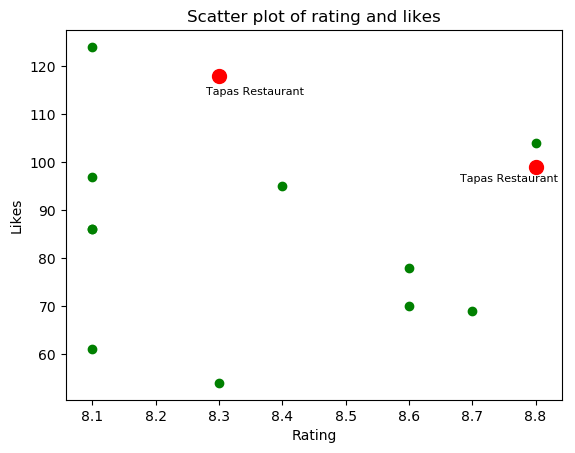
\includegraphics[width=.8\textwidth]{pics/ratings_and_likes}
\end{figure}
  \end{frame}
   % 
    \begin{frame}{The best category}
    \begin{center}
{\bf Tapas Restaurant} is the best choice because:
 \end{center}
\begin{itemize}
\item[\EightStarTaper] one out of two available restaurants has the highest rating;
\item[\EightStarTaper] the other one has the second to largest amount of likes;
\item[\EightStarTaper] fits into description: {\it unusual restaurant with elegant food}.
\end{itemize}
  \end{frame}
 % 
    \begin{frame}{Location of existing Tapas Restaurants}
\begin{figure}[H]
	\centering
	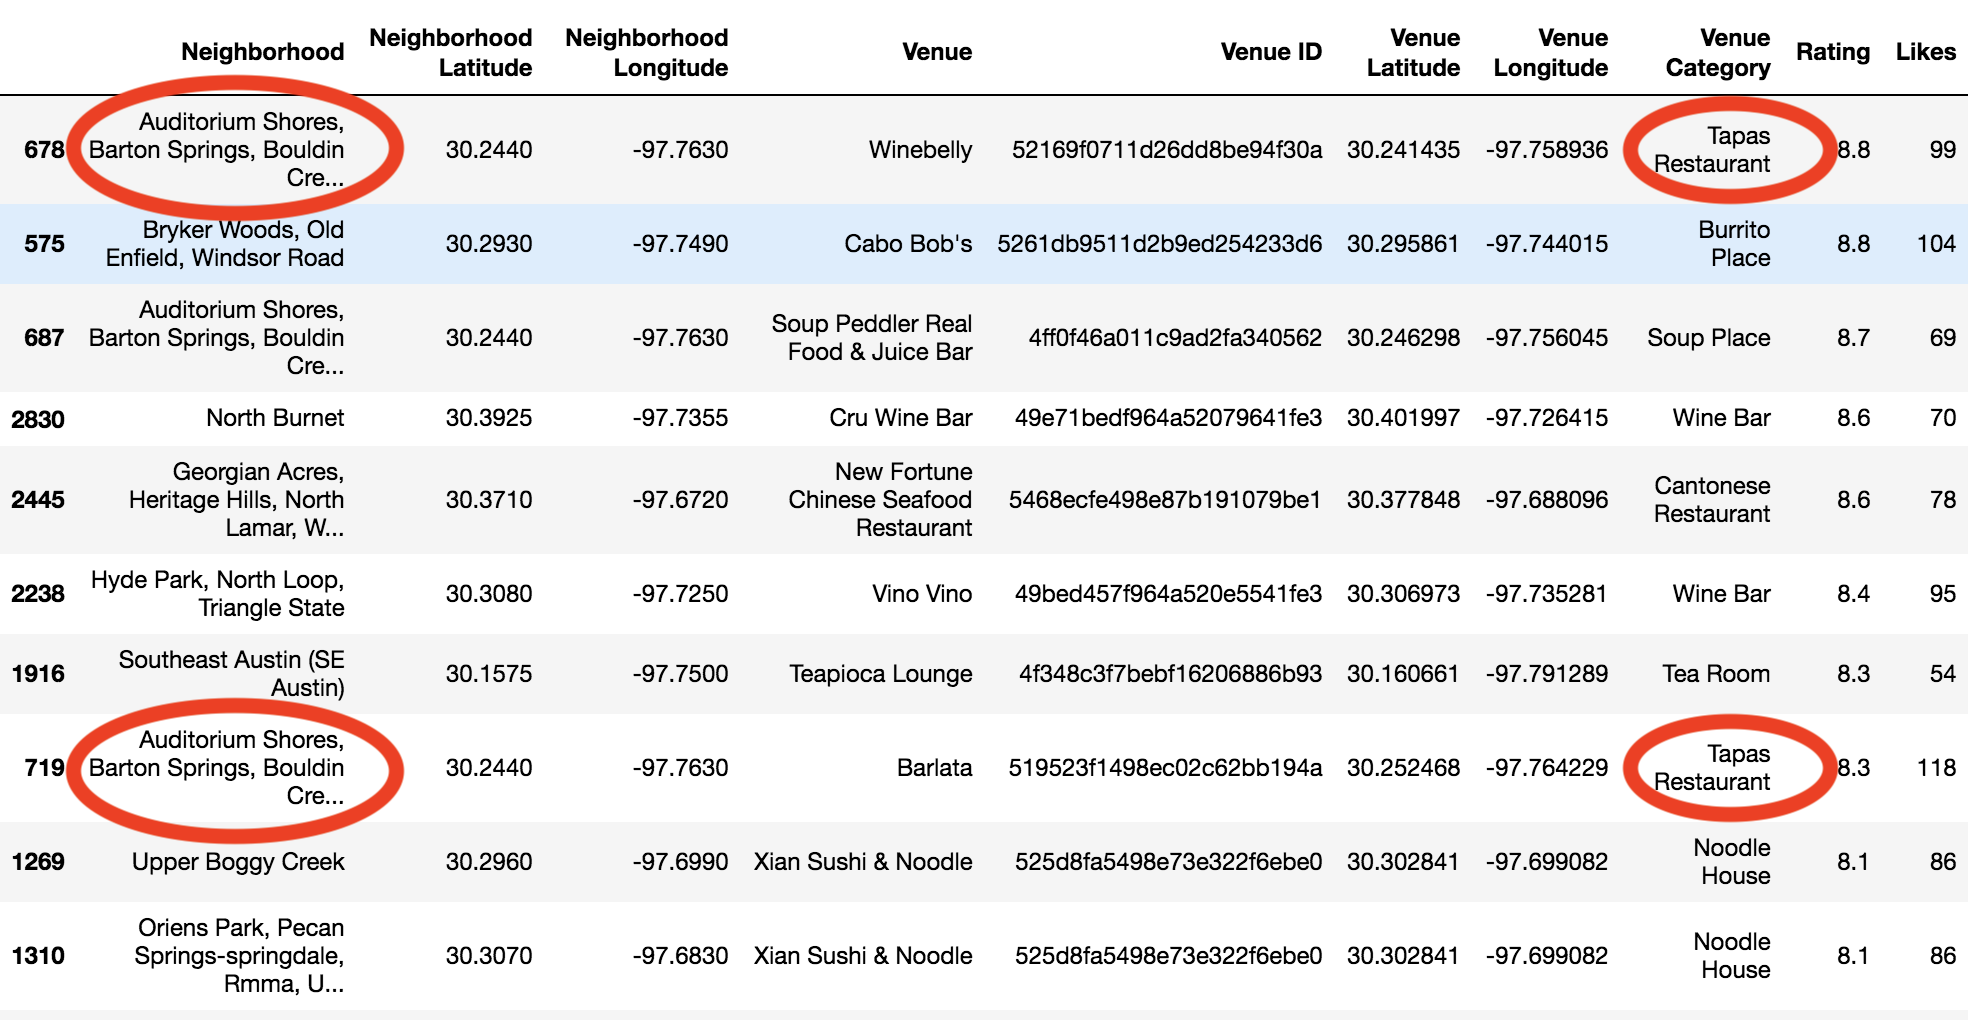
\includegraphics[width=.9\textwidth]{pics/top_10_rare}
\end{figure}
    \begin{itemize}
    \item[\EightStarTaper] both existing Tapas places are located in the same neighborhood;
    \item[\EightStarTaper] to avoid unnecessary competition, find {\it the most similar neighborhood}.
      \end{itemize}
  \end{frame}
  % 
    \begin{frame}{Segmentation of Austin's neighborhoods}
Perform clustering analysis, using k-means algorithm.
    \begin{itemize}
    \item[\EightStarTaper] features include:
    \begin{itemize}
    \item frequencies of all popular venue categories (not limiting to restaurants);
    \item populations and ares of the neighborhoods;
    \end{itemize}
    \item[\EightStarTaper] $k = 7$;
    \item[\EightStarTaper] rescale the features before applying the algorithm for stability.
      \end{itemize}
  \end{frame}
  %
 % 
    \begin{frame}{Segmentation of Austin's neighborhoods (cont'd)}
    Cluster of interest (with the neighborhood in which there are Tapas restaurants) contains three neighborhoods:
\begin{figure}[H]
	\centering
	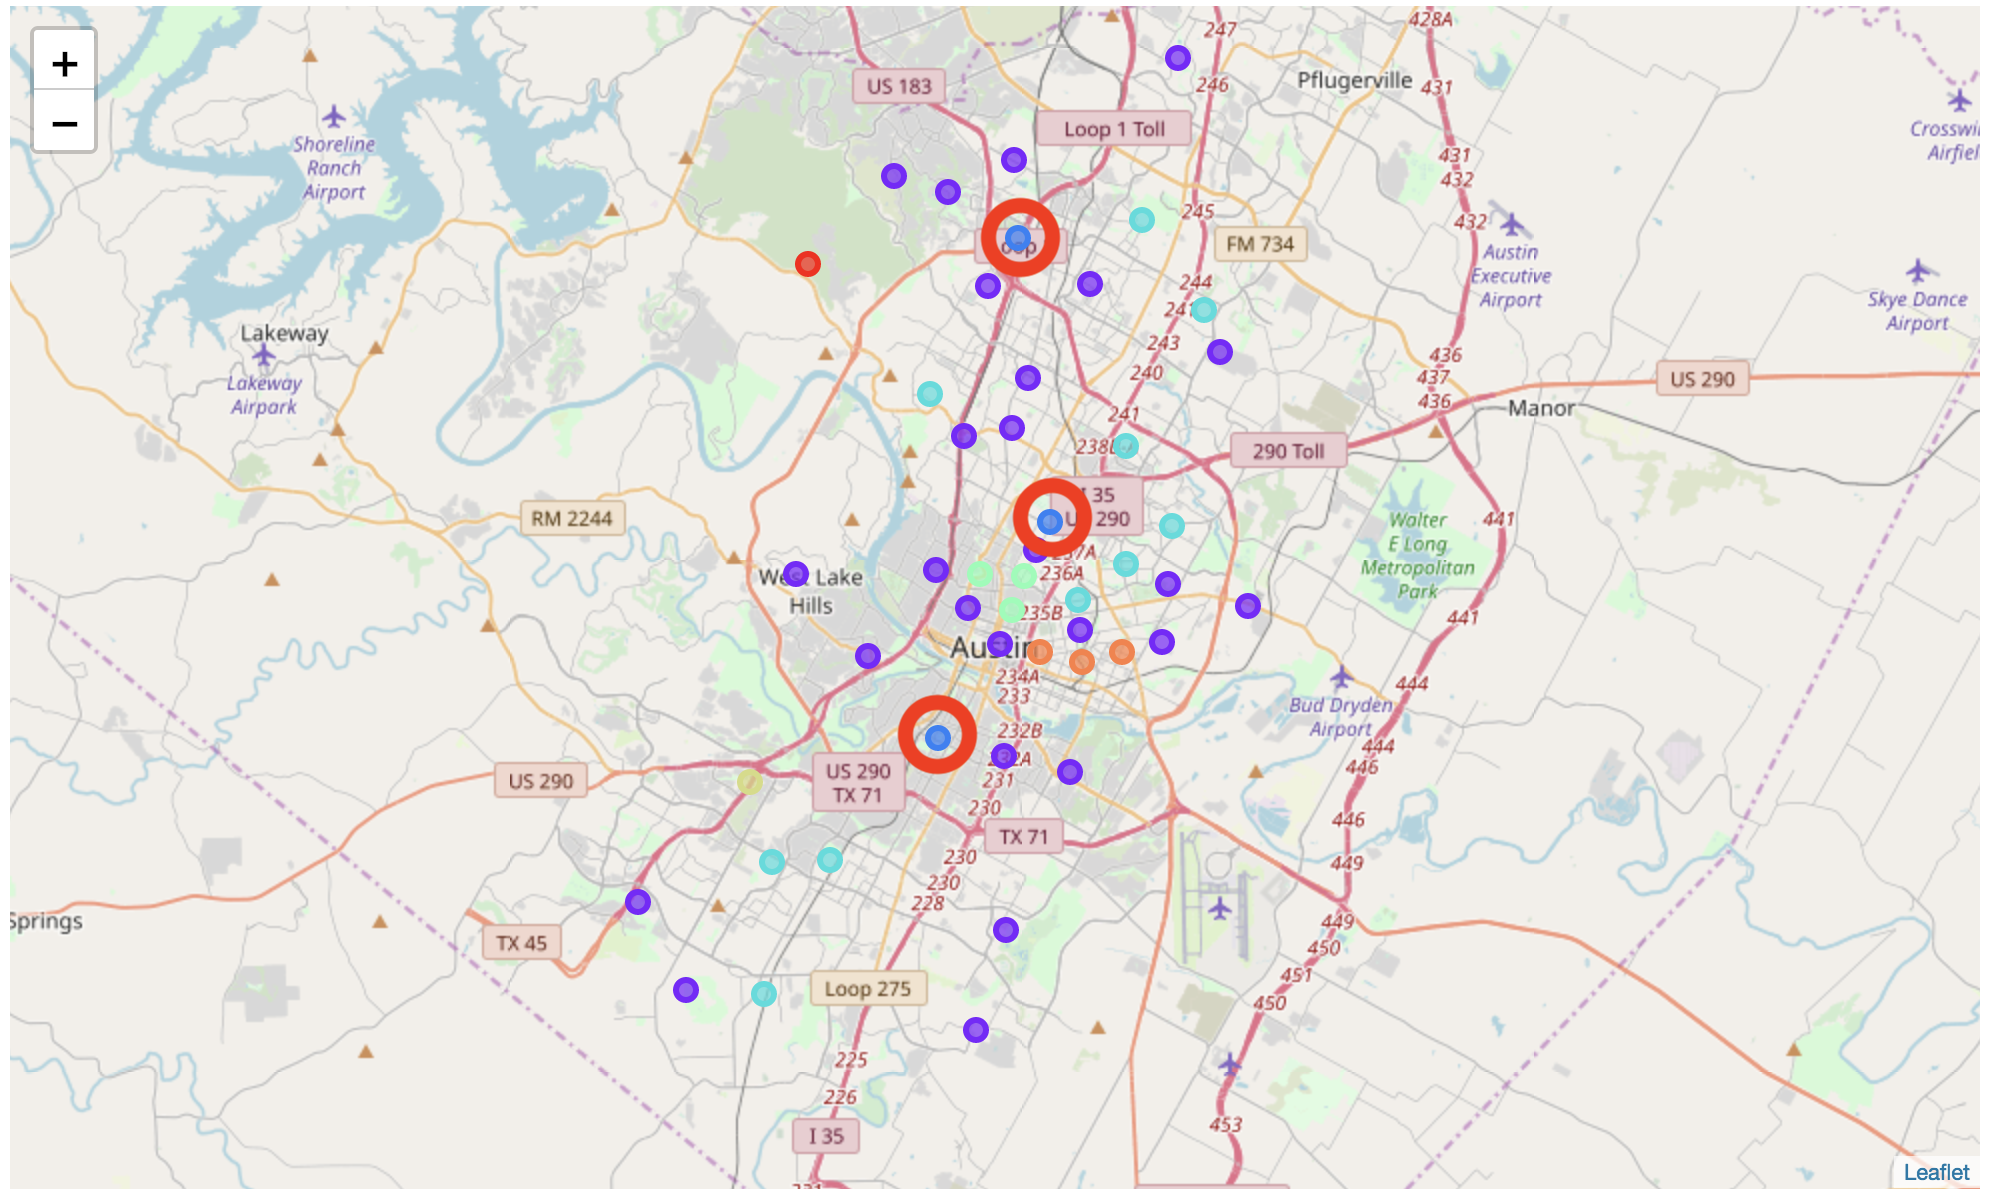
\includegraphics[width=.9\textwidth]{pics/clusters_2}
\end{figure}
  \end{frame}
  % 
    \begin{frame}{The best location}
The optimal possible locations are the two neighborhoods in the cluster of interest, not including the one that already has Tapas Restaurants:
{\bf 
 \begin{itemize}
 \item[\EightStarTaper]
    \begin{itemize} 
    \item[--] Hyde Park$^*$
    \item[--] North Loop$^*$
    \item[--] Triangle State$^*$
    \end{itemize}
    \item[\EightStarTaper] North Burnet
      \end{itemize}
   }
   {\tiny {\it *Note that some neighborhoods contain small sub-nieghborhoods sharing the same zipcodes.}}
   
  {\it Observation: both of neighborhoods have Wine Bars, which is a similar venue category, so a new Tapas Restaurant should fit nicely in such a neighborhood.}
  \end{frame}
 % 
    \begin{frame}{Conclusions}
 \begin{itemize}
 \item[\EightStarTaper] We performed the analysis of Austin's neighborhoods and available restaurants to suggest a new unusual restaurant and the optimal location.
   \item[\EightStarTaper] The best category turned out to be a {\bf Tapas Restaurant} and the best locations:
   {\bf
   \begin{itemize}
   \item Hyde Park
   \item North Loop
   \item Triangle State
   \item North Burnet
   \end{itemize}
   }
   \item Possible improvement of clustering accuracy -- gather more data about nieghborhoods' population.
      \end{itemize}
  \end{frame}
 % 
 
\end{document}

